%	CHAP Docker%----------------------------------------------------------------------------------------

\chapterimage{blue-chapter-head_4-reduced.pdf} % Chapter heading image

\chapter{Instant refresh}\label{chap:Instant refresh}
Instant Refresh (IR) allows users to make changes in their scripts and
get back results immediately by executing the changes on the fly.
Statements in Analysis nodes as well as expressions in RScript nodes are supported
at the moment. The changes are automatically detected and copied to a new Analysis
node called \texttt{Instant refresh}. Based on the settings in the preferences either
a normal run configuration with a local R installation or a new docker container
is started and some basic information is shown in the IR tool. 

\section{Usage}
IR is activated by default but this behavior can be opted out in the preferences.
To allow re-executing code in RScript nodes make sure that you are using
the install or load expression (type \texttt{installOrLoad} and use auto-complete) for loading
r libraries in the script. This expression is needed for locating all the libraries
that need to be loaded when the code is re-executed. It should be used as a
replacement for the R commands \texttt{install.packages} and \texttt{load}.
\begin{remark}
Note that not all expressions are considered changes that need to be re-executed. A few major ignored nodes are
empty lines, comments and save session expressions.
\begin{figure}[h!tbp]
  \centering
  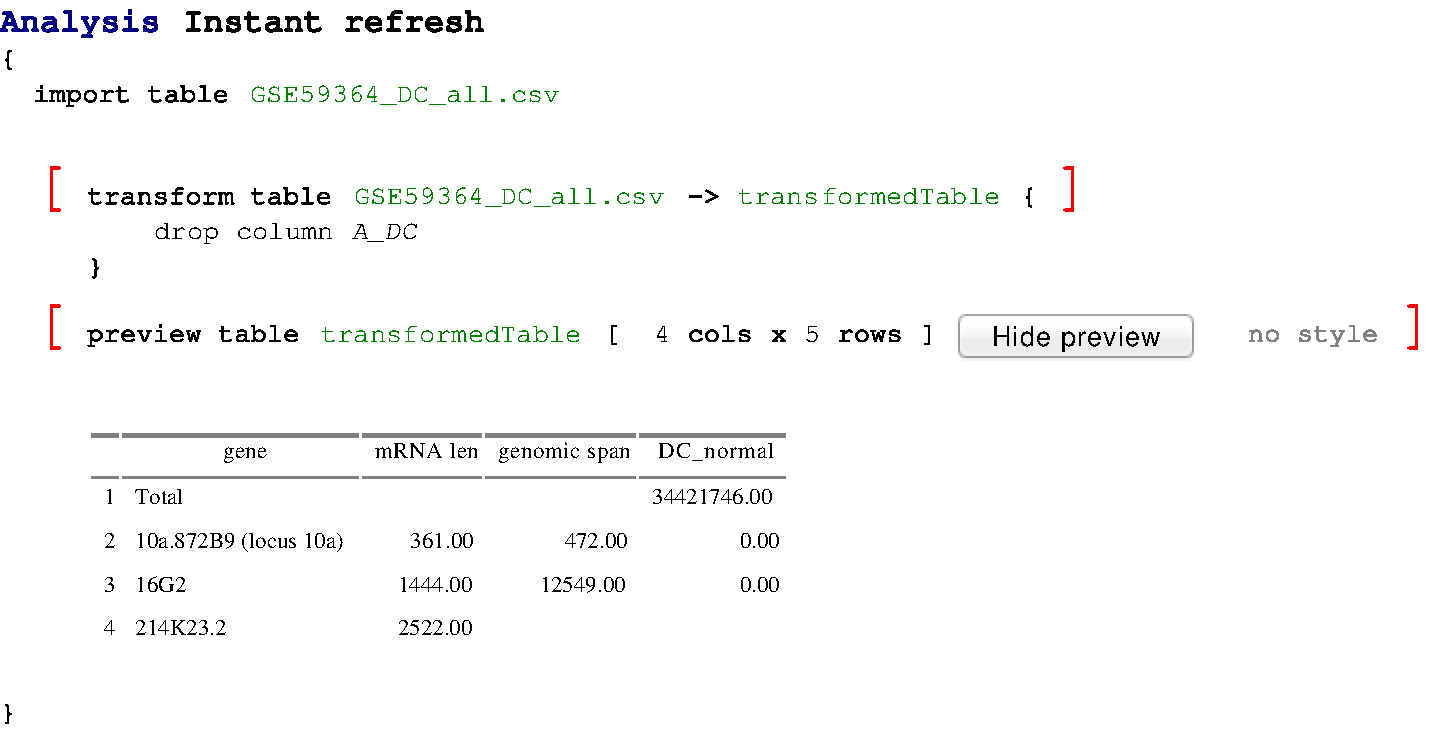
\includegraphics[width=\figWidthWide]{figures/IRChangedStatements.pdf}
\caption[Changed statements in an Analysis node]{\textbf{Changed statements in an Analysis node} A change was made in the transform table statement and all statements that need to be re-executed are surrounded by red brackets.}
\end{figure}

\subsection{Instant refresh node}
The Analysis node \texttt{Instant refresh} is a node that is automatically inserted in the current model and is populated with all expressions/statements
that have to be re-executed. Changes that are made in this node are not automatically detected and are overridden the next time IR is executed.

\section{IR Preferences}
The preferences can be found in the Preferences/Settings MPS menu(\menu{MPS > Preferences > Other Settings > InstantRefresh} on Mac, \menu{MPS > Settings >  Other Settings} \menu{ > InstantRefresh} on PC). \newline There are a few options that can be changed:

\begin{enumerate}

\begin{figure}[h!tbp]
  \centering
  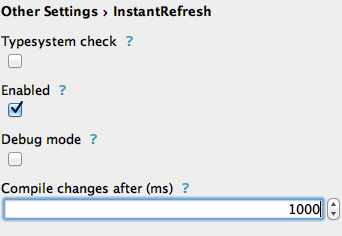
\includegraphics[width=\figWidthNarrow]{figures/IRPreferences.png}
\caption[IR preferences]{\textbf{IR preferences} This dialog is available under MPS Preferences/Settings.}
\end{figure}

	\item \textbf{Type system check}. 
	If this option is enabled, instant refresh is not executed when the type system 	reports errors for the current node.
	\item \textbf{Enabled}. Toggle this option to activate or deactivate IR.
	\item \textbf{Debug mode}.
	Toggles the visibility of additional messages in the IR tool. These messages 			are helpful for debugging purposes.
	They also give some additional information why in some cases IR was not 		executed (e.g. the feature is not enabled, a pause expression is active..).
	Additionally it outputs the standard output of the currently executing script 	that would normally be found in the Run tab console.

\end{enumerate}

\section{Tool}
The IR tool is a tab that is located at the bottom left of the screen. It displays a message when R code is generated and executed as
well as the execution time of both of these phases. If the debugging mode is activated, the output is way more verbose.

\section{Pause instant refresh}
Although IR can be disabled in the preferences, there is sometimes a need to pause it only for the current script. RScript nodes have
a built-in expression to achieve this. It can be activated by typing \texttt{pause instant refresh} and using auto-complete anywhere in the script.
This expression can only be used once per script because it affects the whole script.

\section{Sessions}
To accelerate the re-execution of R code, sessions are used. Sessions are files with the extension ".RDa" and are saved in a sub folder of the results directory.
They contain an external representation of R objects that can be used for restoring the r environment. Every statement in an Analysis node automatically saves
a new session file after the execution of the statement. In RScript nodes save session expressions can be inserted manually. They can only be inserted at the
root level of the script and not inside nested expressions (e.g. if statements, functions, blocks...). When a change is made, the nearest saved session is loaded
and changed expressions are only executed if they are located after this expression. All sessions in the current model can be removed by using the use the "Invalidate Sessions" intention (\intentionLightBulb)
 and new session files will be created on the next run of IR.
\begin{figure}[h!tbp]
  \centering
  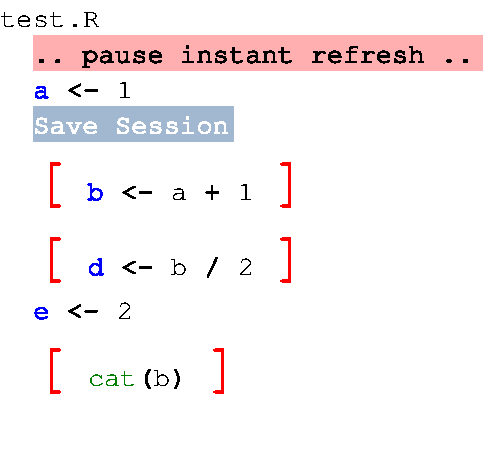
\includegraphics[width=\figWidthNarrow]{figures/IRPauseAndSessionExpression.pdf}
\caption[Sessions affect the list of changed nodes]{A change was made in the expression after the save session expression and therefore the line above doesn't have to be re-executed.}
\end{figure}
\end{remark}